%!TEX root = report.tex

\subsection{Experimental Results}

\begin{figure}[H]
    \centering
    \begin{subfigure}{0.49\linewidth}
        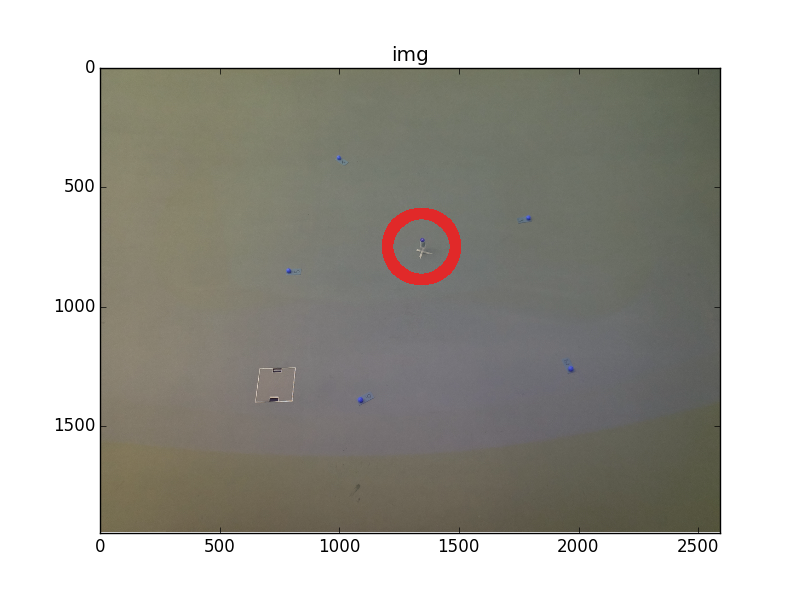
\includegraphics[width=\linewidth]{files/res0_img139.png}
        \caption{View of camera 139 with reference points and target point}
    \end{subfigure}
    \begin{subfigure}{0.49\linewidth}
        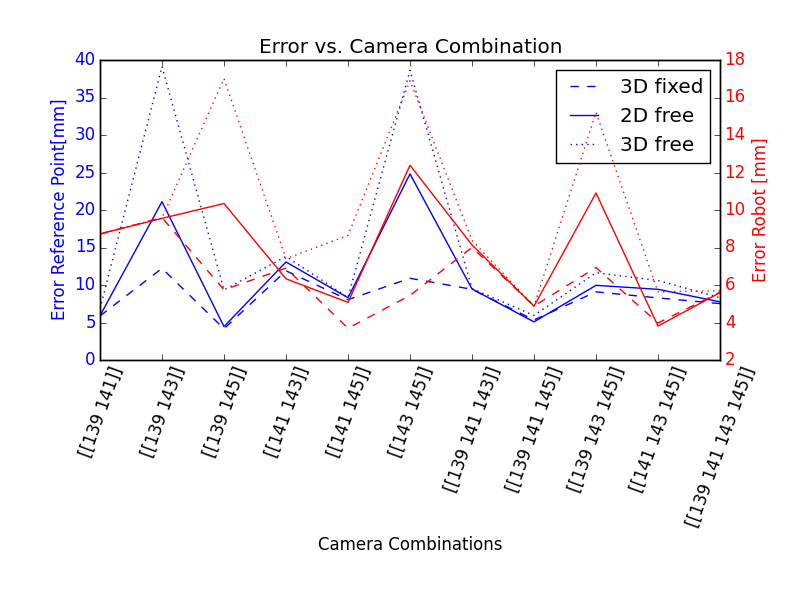
\includegraphics[width=\linewidth]{files/res0_combi_4.png}
        \caption{2D and 3D errors of 4th reference point and robot}
    \end{subfigure}
    \caption{Results of experiment in Atrium}
    \label{fig:experiment0}
\end{figure}

\begin{figure}[H]
    \centering
    \begin{subfigure}{0.49\linewidth}
        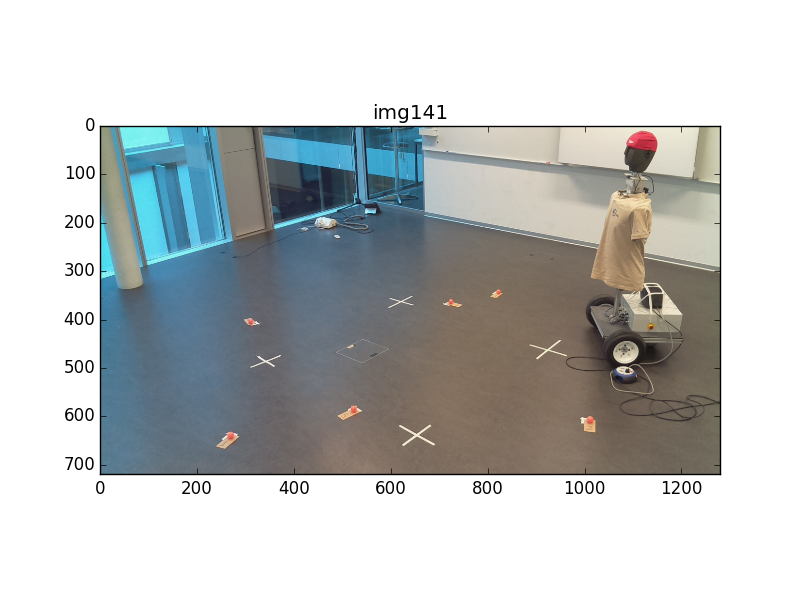
\includegraphics[width=\linewidth]{files/res1_img141.png}
        \caption{View of camera 141 with reference points and robot}
    \end{subfigure}
    \begin{subfigure}{0.49\linewidth}
        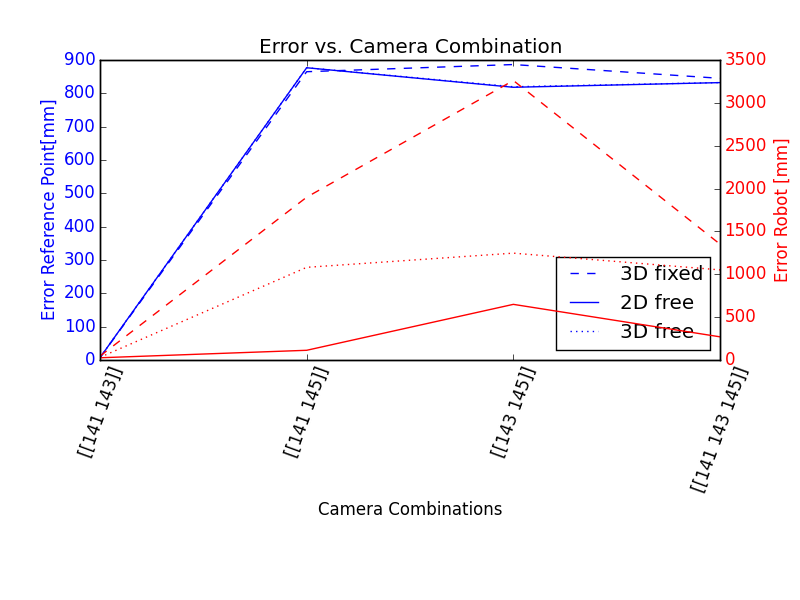
\includegraphics[width=\linewidth]{files/res1_combi_4.png}
        \caption{2D and 3D errors of 4th reference point and robot}
    \end{subfigure}
    \begin{subfigure}{0.6\linewidth}
        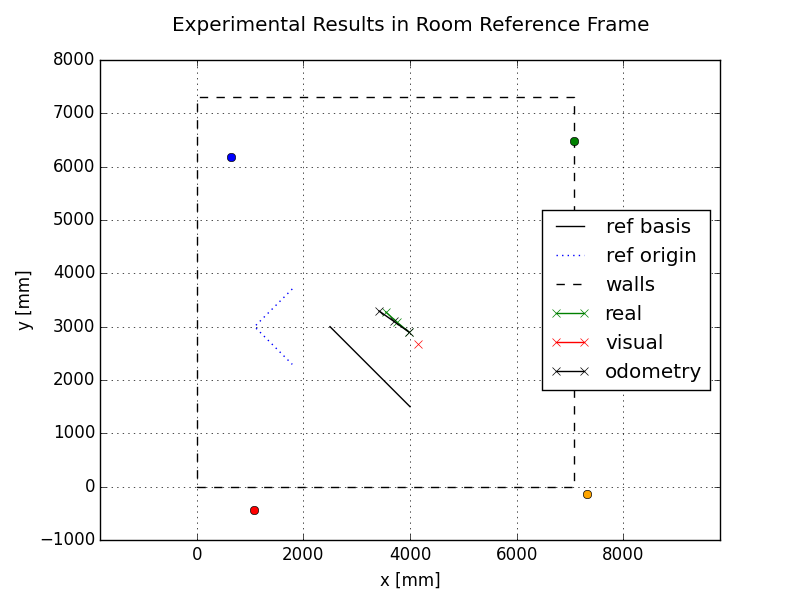
\includegraphics[width=\linewidth]{files/res1_room.png}
        \caption{Summary of results in room reference frame}
    \end{subfigure}
    \caption{Results of experiment 1 in BC329 (Camera numbering: blue 139, red 141, green 143, orange 145)}
    \label{fig:experiment1}
\end{figure}

\begin{figure}[H]
    \centering
    \begin{subfigure}{0.49\linewidth}
        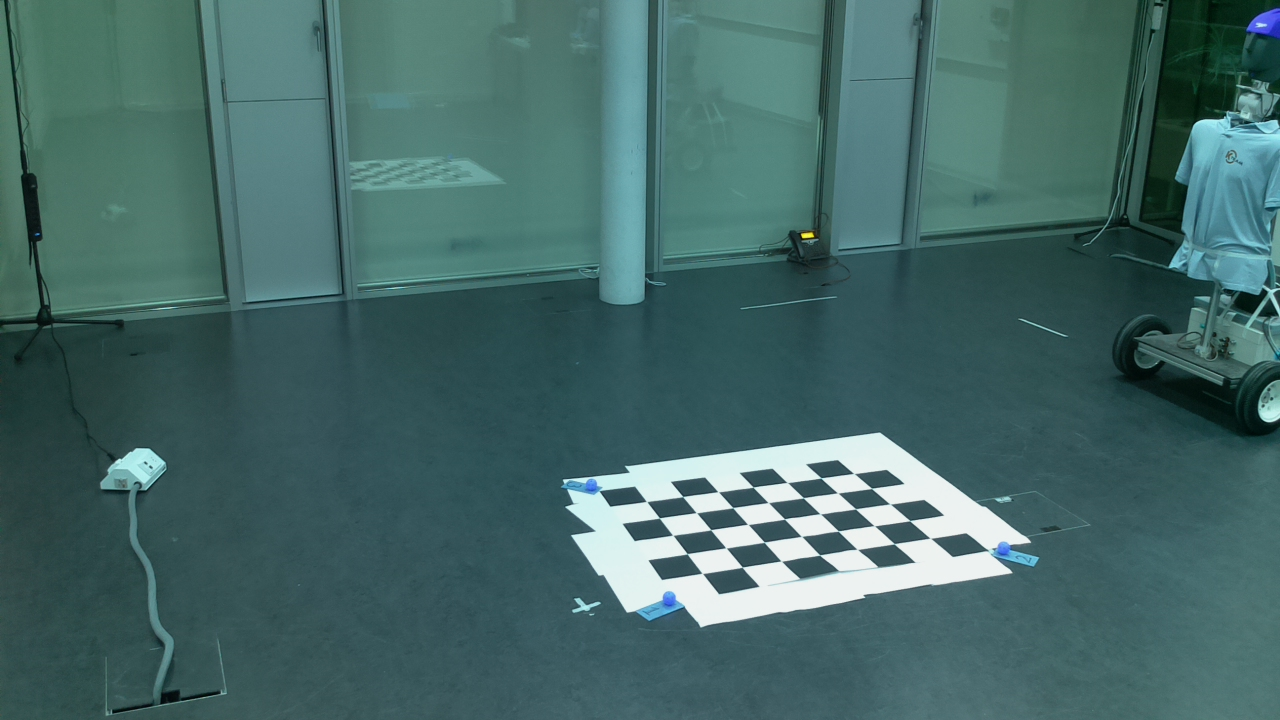
\includegraphics[width=\linewidth]{files/res2_image_143.png}
        \caption{View of camera 143 with checkerboard}
    \end{subfigure}
    \begin{subfigure}{0.49\linewidth}
        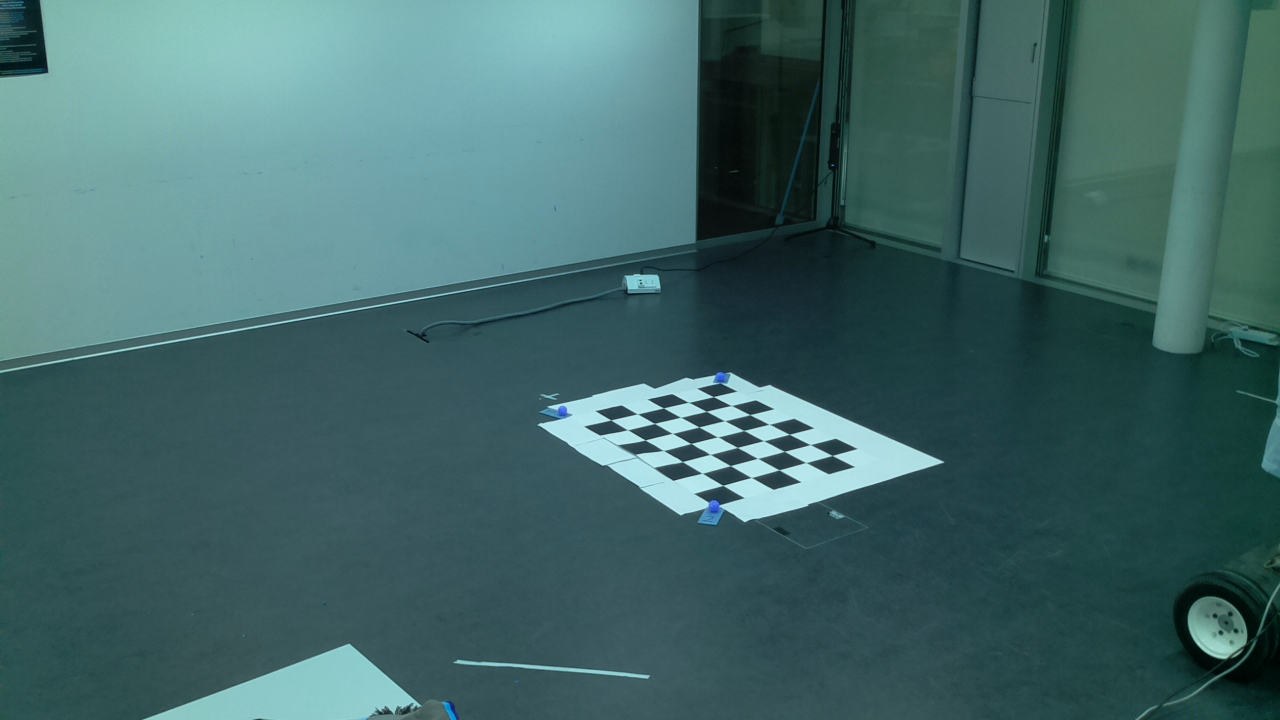
\includegraphics[width=\linewidth]{files/res2_image_145.png}
        \caption{View of camera 145 with checkerboard}
    \end{subfigure}
    \begin{subfigure}{0.49\linewidth}
        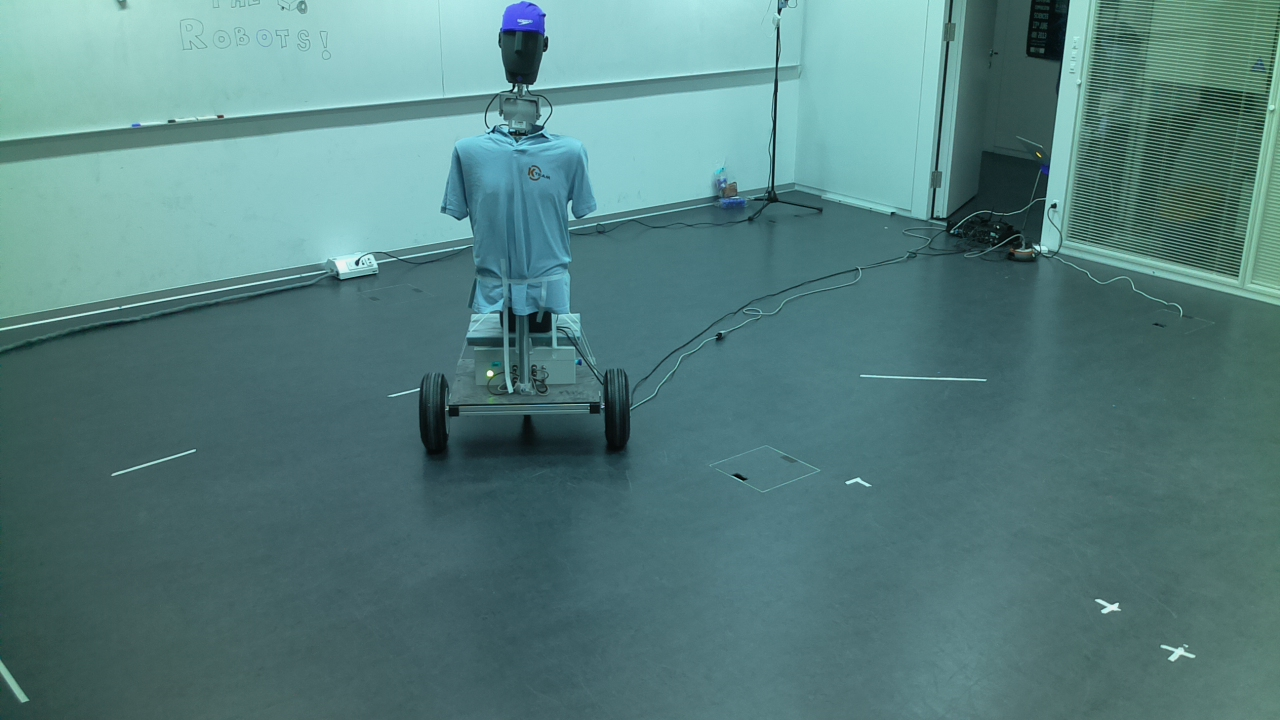
\includegraphics[width=\linewidth]{files/res2_0_image_141.png}
        \caption{View of camera 141 with robot}
    \end{subfigure}
    \begin{subfigure}{0.49\linewidth}
        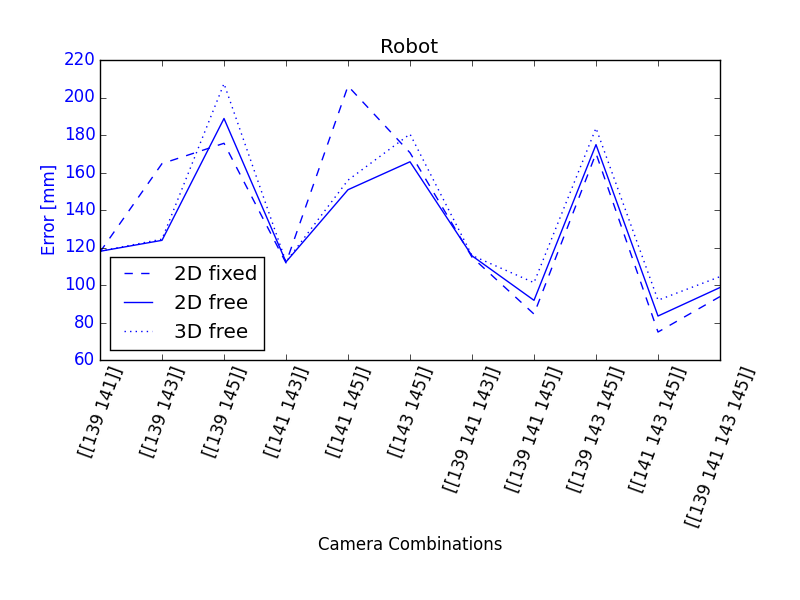
\includegraphics[width=\linewidth]{files/res2_combi_rob.png}
        \caption{2D and 3D errors of robot}
    \end{subfigure}
    \begin{subfigure}{0.6\linewidth}
        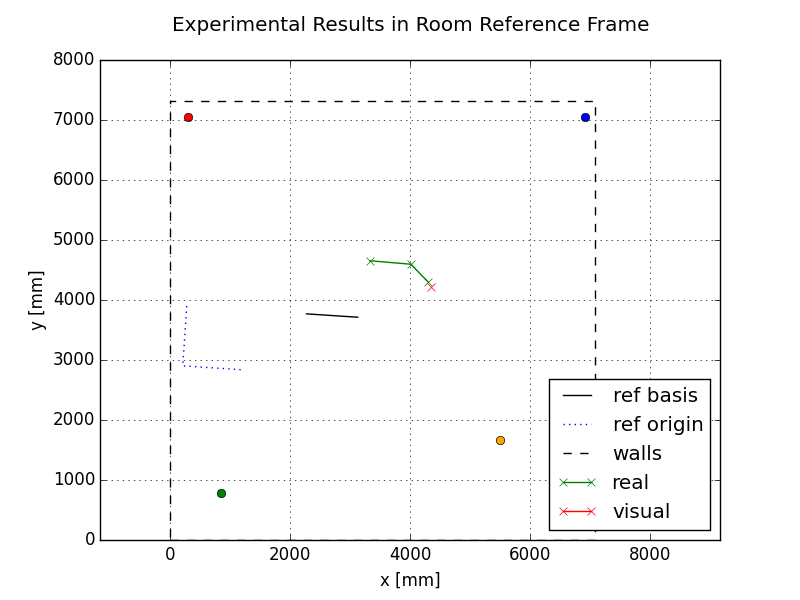
\includegraphics[width=\linewidth]{files/res2_room.png}
        \caption{Summary of results in room reference frame}
    \end{subfigure}
    \caption{Results of experiment 2 in BC329 (Camera numbering: blue 139, red 141, green 143, orange 145)}
    \label{fig:experiment1}
\end{figure}




